%課題研究レジュメテンプレート ver. 1.2

\documentclass[uplatex]{jsarticle}
\usepackage[top=20mm,bottom=20mm,left=20mm,right=20mm]{geometry}
\usepackage[T1]{fontenc}
\usepackage{txfonts}
\usepackage{wrapfig}
\usepackage[expert,deluxe]{otf}
\usepackage[dvipdfmx,hiresbb]{graphicx}
\usepackage[dvipdfmx]{hyperref}
\usepackage{pxjahyper}
\usepackage{secdot}

\makeatletter
  \renewcommand{\section}{%
    \if@slide\clearpage\fi
    \@startsection{section}{1}{\z@}%
    {\Cvs \@plus.5\Cdp \@minus.2\Cdp}% 前アキ
    {.5\Cvs \@plus.3\Cdp}% 後アキ
    %{\normalfont\Large\headfont\raggedright}}
    {\normalfont\raggedright}}

  \renewcommand{\subsection}{\@startsection{subsection}{2}{\z@}%
    {\Cvs \@plus.5\Cdp \@minus.2\Cdp}% 前アキ
    {.5\Cvs \@plus.3\Cdp}% 後アキ
    %{\normalfont\large\headfont}}
    {\normalfont}}

  \renewcommand{\subsubsection}{\@startsection{subsubsection}{3}{\z@}%
    {\Cvs \@plus.5\Cdp \@minus.2\Cdp}%
    {\z@}%
    %{\normalfont\normalsize\headfont}}
    {\normalfont}}
\makeatother
%ここから上を編集する必要はない.





\title{\vspace{-14mm}Redpenを使った文書自動添削ツール}
\author{PMコース 矢吹研究室 1442031 氏名 小山 隆太郎}
\date{}%日付を入れる必要はない.
\pagestyle{empty}%ページ番号は振らない.
\begin{document}
\maketitle





\section{研究の背景}
ソフトウェアエンジニアはプログラムを組むだけではなく,たくさんの技術文書を書く.そして専門的なチュートリアル,マニュアル等を読み手に理解してもらうことが大切である.ソフトウェアを開発する際には多くの実装テストをする必要がある.そのためCheckStyleやlint等の静的解析ツールを導入することで,フォーマットのエラーを自動で検知することが出来る.しかし静的解析ツールは文書のチェックを行えるものがなく,文中のミスを修正することに時間を割く等で作業の本質に取り組む時間以外に無駄が生じてしまうことがある.このことはエンジニアにとって悩みの種である.このような状況に対してRedpenと呼ばれる文書静的解析ツールが開発され,日々エンジニアが改良を加えている\cite{a}.Redpenは一部の静的解析ツール(CheckStyle,lint等)に相当する機能を文書に与えるものであり,文書作成でも最低限の検査を自動で行いたいという動機の下,改良が進んでいる.大学の授業等で文書を提出することがあるため,Redpenの開発に着目することでこれからの文書作成の質が向上するのではないかと考えた.

\section{研究の目的}
Redpenを利用し,文書作成に割く時間を短縮できるようにすることで,もっと大きな粒度の問題(実作業,着目すべき文や質等)に集中できるようにすることが目的である.また,文中のミスを少なくした状態で文書を提出できるようにする\cite{b}.

\section{研究の手法}
\begin{itemize}
 \item1,Redpenが動作する環境を構築する\cite{c}.
 \item2,動作することを確認したら,日本語の文書”ja”が添削できるように設定ファイルを書き換える.
 \item3,参考文献のサンプル文\cite{d}で添削を行い,添削結果が本の改善文に準拠するよう設定ファイルを書き換える. 
\end{itemize}

\section{研究の結果}
Redpenの設定ファイルを書き換え,以下の表現を添削する機能にした.
\begin{itemize}
 \item SuccessiveWord 同一の単語が連続して使用されていないかを検査する.
 \item KatakanaEndHyphen カタカナ単語末尾の長音検査する.
 \item KatakanaSpellCheck カタカナ単語のスペルチェックをする.
 \item InvalidExpression 顔文字や感情的な表現など技術文書で利用するべきでない句の使用を検査する.
 \item JapaneseStyle ですます調,である調が混じっていないかを検査する.
 \item DoubleNegative 二重否定を検知する.
 \item FrequentSentenceStart 同じ文頭表現が過度に利用されていないか検査する.例えばどの文頭も”私は〜”からはじまる等.
 \item JapaneseAmbiguousNounConjunction 格助詞の「の」+名詞連続+格助詞の「の」というパターンを発見するとエラーを出力する.
 \item JapaneseNumberExpression 日本語の数値表現を検査する機能.「ひとつ,ふたつ」,「1つ,2つ」などのゆらぎを検知する.
 \item LongKanjiChain 長過ぎる漢字の連続をみつけるとエラーを出力する.
 \item SuccessiveSentence 同一内容の文が連続して出現するとエラーを出力する.
 \item DoubledConjunctiveParticleGa 一文に二回以上,接続助詞または二重否定の「が」が出現するとエラーを出力する.
\end{itemize}

Redpenがコマンド上で動作し,文中ミスを正しく抽出できたので以下に実行結果を載せる.

%\begin{wrapfigure}[行数]{r}{幅}%行数はオプションだが,調整しないとうまくいかない.
\begin{figure}[htb]
\centering
%\vspace*{-\intextsep}
%\includegraphics[width=図の幅,clip]{ファイル名}\label{参照用ラベル}
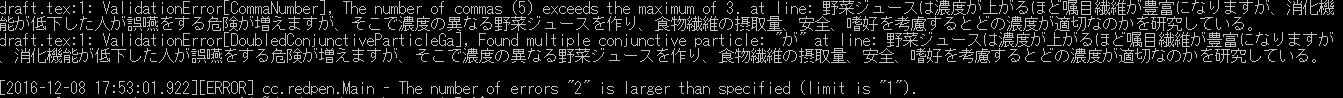
\includegraphics[width=16cm,clip]{image1.png}
\caption{}\label{サンプル図}
\end{figure}

図1は2ヶ所の文中ミスを指摘している.ValidationError[CommaNumber] The number of commas (5) exceeds the maximum of 3. at lineは文中の句点(コマ数)が多いことを指摘している.この場合” 摂取量、安全、嗜好”の句点を”・”にすることで見やすい表記になる.ValidationError[DoubledConjunctiveParticleGa], Found multiple conjunctive particle: "が" at lineは文中に二重否定があることを指摘している.この場合”野菜ジュースは濃度が上がるほど嘱目繊維が豊富になりますが 、消化機能が低下した人が誤嚥をする危険が増えますが、”と二重否定が使われていることがわかる.

%\begin{wrapfigure}[行数]{r}{幅}%行数はオプションだが,調整しないとうまくいかない.
\begin{figure}[htb]
\centering
%\vspace*{-\intextsep}
%\includegraphics[width=図の幅,clip]{ファイル名}\label{参照用ラベル}
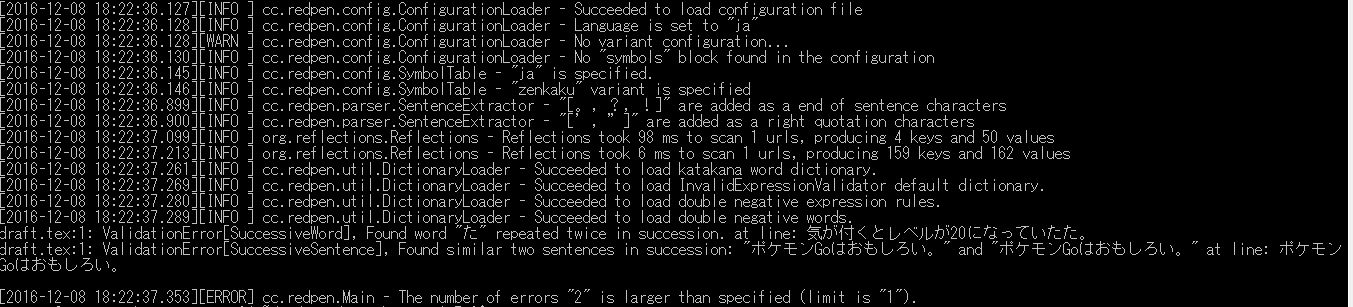
\includegraphics[width=16cm,clip]{image2.png}
\caption{}\label{サンプル図}
\end{figure}

図2は2ヶ所の文中ミスを指摘している.ValidationError[SuccessiveWord], Found word "た" repeated twice in succession. at line:は文末の”た”が2つあることを指摘している.ValidationError[SuccessiveSentence], Found similar two sentences in successionは文中に同じパラグラフが2つあることを指摘している.この場合”ポケモンGoはおもしろい。”が2つあることを指摘している.

\section{考察と今後の計画}
Redpenには設定ファイルが設けられており,設定を書き換えるごとに出力結果も変わる.その為きちんとした設定が確立されておらず,現在も研究が続いている.Redpenのファイルの設定を確立し,文中のミスを抽出することは出来たが,中には不要である間違いを指摘されることがあった.これを取り除く設定を確立できれば,より精度の高い文書添削ツールになり得るだろう.今後は皆が共通して使えるように添削マシンを拡張する予定である.


\bibliographystyle{junsrt}
\bibliography{biblio}%「biblio.bib」というファイルが必要.

\end{document}
